\documentclass[oneside]{memoir}

\usepackage{lmodern}
\usepackage[T1]{fontenc}
\usepackage[spanish,activeacute]{babel}
\usepackage{mathtools}
\usepackage{graphicx}
\usepackage{titlesec}

\titleformat{\chapter}[display]
  {\normalfont\bfseries}{}{0pt}{}

\title{YourPlacesBot - A Telegram Bot}
\author{David Quesada L\'opez y Mateo Garc\'ia Fuentes}

\setlength{\parskip}{1em}

\newcommand{\romanpages}{
\pagenumbering{roman}
\thispagestyle{empty}
\beforepartskip
\centering

\thetitle

\theauthor

GRADO EN INGENIER\'IA INFORM\'ATICA 

FACULTAD DE INGENIER\'IA INFORM\'ATICA

UNIVERSIDAD COMPLUTENSE DE MADRID


\includegraphics{logo.jpg}

TRABAJO DE FIN DE GRADO EN INGENIER\'IA INFORM\'ATICA

Director: Carlos Gregorio Rodr�guez

\today
\afterpartskip
\newpage

\thispagestyle{empty}
%\beforepartskip
\raggedright

\begin{center}
  \makebox{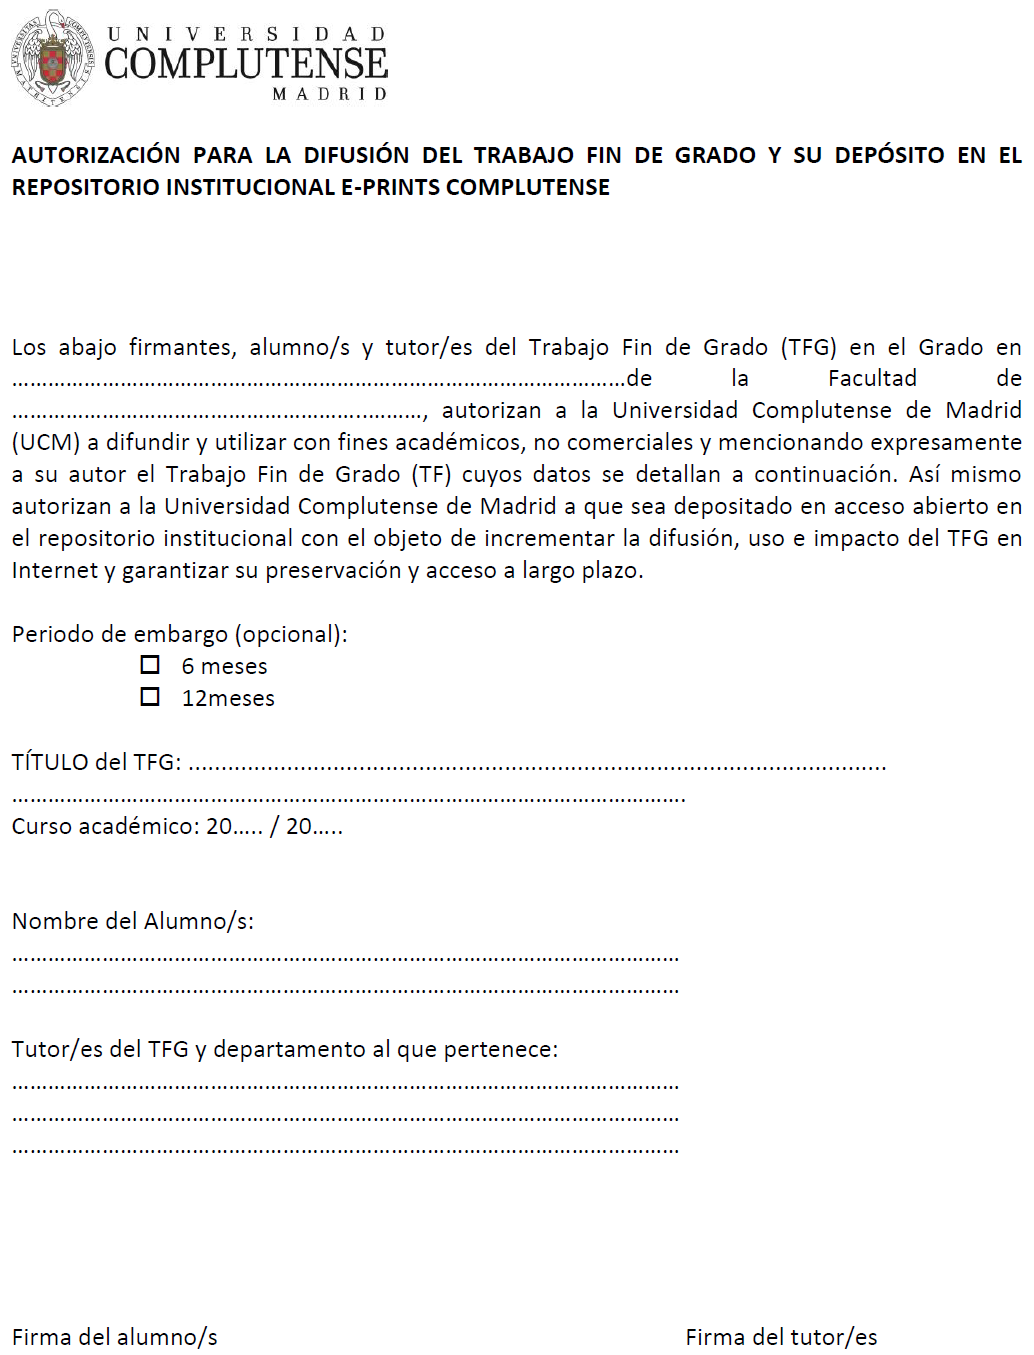
\includegraphics[width=\textwidth]{autoriz.png}}
\end{center}

\afterpartskip
\newpage
\thispagestyle{empty}
\raggedright

\textbf{Agradecimientos}

Gracias a Nick Lee (https://github.com/nickoala) por desarrollar telepot, un framework de Python para API de Telegram Bot y desarrollarlo bajo una licencia MIT.

\afterpartskip
\newpage
}

\newcommand{\indexpage}{
\frontmatter
\setcounter{page}{4}
\pagestyle{plain}

\tableofcontents

\newpage
}


\begin{document}
\romanpages
\indexpage

\mainmatter

\newpage
\chapter[\'Indice de figuras]{\'Indice de figuras}

\newpage
\chapter[\'Indice de abreviaturas]{\'Indice de abreviaturas}

\newpage
\chapter[Resumen]{Resumen}
Una de los principales atractivos de Telegram es su plataforma para bots. Los usuarios pueden crear sus propios bots y ponerlos en funcionamiento para que sean accesibles a todos los clientes de Telegram sin coste alguno para el desarrollador o para el consumidor. Estos bots proporcionan en su mayor�a informaci�n, juegos o utilidades dentro de un chat, y aumentan en gran medida la funcionalidad de Telegram.

A la hora de que un usuario interact�e con un bot, es especialmente interesante que el servicio que se le preste pueda depender de su ubicaci�n geogr�fica y pueda tener un componente social. Por ello, este proyecto tiene como objetivo informar al usuario sobre qu� establecimientos cercanos hay en base a su localizaci�n, ofreciendo la posibilidad de encontrarlos f�cilmente y de ver datos proporcionados por otros usuarios sobre estos.



Palabras clave: bot, Telegram, geolocalizaci�n, noSQL, 

\newpage
\chapter[Abstract]{Abstract}
One of the main features of Telegram is its bot support. Users can create their own bots and launch them to be available for everyone in Telegram without cost for neither the developer nor the client. These bots mainly offer information, games or utilities inside the chat and they increase greatly Telegrams functionality.

When an user interacts with a bot, it is of special interest that the response of the bot varies depending on the users location and on a social component. That's why this project aims to inform the user about what near by establishments there are depending on his location, offering the posibility to find them easily and to see information of them given by other users.

Keywords: bot, Telegram, geolocation, noSQL,

\newpage
\chapter[Cap\'itulo 1: Introducci\'on]{Cap\'itulo 1: Introducci\'on}

\newpage
\chapter[Cap\'itulo 2: Materiales y m\'etodos]{Cap\'itulo 2: Materiales y m\'etodos}

\newpage
\chapter[Cap\'itulo 3: Resultados]{Cap\'itulo 3: Resultados}

\newpage
\chapter[Cap\'itulo n: Conclusiones]{Cap\'itulo n: Conclusiones}

\newpage
\chapter[Ap\'endice]{Ap\'endice}

\newpage
\begin{thebibliography}{}
%Falta escribirlo en formato IEEE
\bibitem
*LaTex -> http://texdoc.net/texmf-dist/doc/latex/memoir/memman.pdf 
\bibitem
*Python -> https://docs.python.org/2.7/
\bibitem
*API Google Maps Docs -> http://googlemaps.github.io/google-maps-services-python/docs/2.4.5/
\bibitem
*Telegram Bots -> https://core.telegram.org/bots
\bibitem
*API Telepot -> http://telepot.readthedocs.io/en/latest/
\end{thebibliography}

\newpage
\chapter[Anexo]{Anexo}

\newpage
\chapter[Glosario]{Glosario}

\end{document}